% Measuring Detection Latency in Video World Models
%
% Build:  tectonic paper/main.tex      (or: pdflatex twice)
% Numbers: every figure, table and numeric sentence is generated into
%          paper/generated/ by scripts/make_paper.py. Do not hand-edit them.
%
% To target TMLR, drop tmlr.sty next to this file and replace the geometry/
% font block below with \usepackage{tmlr}. Nothing else needs to change.
\documentclass[11pt]{article}

\usepackage[utf8]{inputenc}
\usepackage[T1]{fontenc}
\usepackage{lmodern}
\usepackage[margin=1.15in]{geometry}
\usepackage{amsmath,amssymb,amsthm}
\usepackage{booktabs}
\usepackage{graphicx}
\usepackage{xcolor}
\usepackage{microtype}
\usepackage{caption}
\usepackage[hidelinks]{hyperref}
\usepackage{natbib}
\bibliographystyle{plainnat}
\usepackage{draftwatermark}
\SetWatermarkText{DRAFT --- results pending}
\SetWatermarkScale{0.28}
\SetWatermarkColor[gray]{0.92}

\captionsetup{font=small,labelfont=bf}
\newcommand{\dt}{\Delta t}
\newcommand{\RMTA}{\ensuremath{\mathrm{RMDL}}}   % restricted mean detection latency
\newcommand{\code}[1]{\texttt{\small #1}}
\newcommand{\pending}{\textcolor{red!70!black}{\textbf{[pending registered run]}}}

\newcommand{\lgwHasResults}{1}
\newcommand{\lgwModel}{\texttt{facebook/vjepa2-vitl-fpc64-256}}
\newcommand{\lgwNAnom}{1000}
\newcommand{\lgwNCalib}{100}
\newcommand{\lgwNEval}{100}
\newcommand{\lgwDim}{1024}
\newcommand{\lgwNBoot}{2000}
\newcommand{\lgwVerdict}{\textsc{negative result}}
\newcommand{\lgwEarlyWarners}{none}
\newcommand{\lgwRmtaWarners}{none}
\newcommand{\lgwMedianDegenerate}{no}
\newcommand{\lgwBaselinesAtChance}{none}
\newcommand{\lgwVacuous}{no}
\newcommand{\lgwSource}{\texttt{results/phase2-20261010-174237/analysis/results.json}}
\newcommand{\lgwNote}{Phase 2: frozen V-JEPA 2, pre-registered protocol.}

\newcommand{\lgwOccFullyHidden}{77.5\%}
\newcommand{\lgwOccPartial}{17.2\%}
\newcommand{\lgwOccFullyHiddenClips}{28.0\%}
\newcommand{\lgwOccluderArea}{29.9\%}

\newcommand{\lgwPilotCalib}{40}
\newcommand{\lgwPilotEval}{0}
\newcommand{\lgwPilotAnom}{68}
\newcommand{\lgwPilotTotal}{108}
\newcommand{\lgwPilotTarget}{280}
\newcommand{\lgwPilotState}{in progress; control clips incomplete, so no thresholds can be calibrated and no result can yet be computed from it}

\newcommand{\lgwPrecWorstProbeBf}{6.74\%}
\newcommand{\lgwPrecWorstLossBf}{0.23\%}
\newcommand{\lgwPrecRatioBf}{30}


\title{\bfseries Measuring Detection Latency in Video World Models:\\
A Pre-Registered Protocol and Its Failure Modes\\[4pt]
\large\normalfont\textcolor{red!70!black}{DRAFT --- results pending registered run}}
\author{Anonymous Author(s)}
\date{}

\begin{document}
\maketitle

\begin{center}
\fcolorbox{red!60!black}{red!5}{\parbox{0.93\linewidth}{\small
\textbf{Results pending.} The registered experiment has not been run: it
requires GPU credit that was not available, not any missing code. The harness is
complete, tested and launch-ready at an estimated one GPU-hour. Every place a
registered number would appear is marked \pending{} and no placeholder,
estimated or illustrative value appears anywhere in this manuscript. This
version contributes the protocol, the benchmark and the failure modes we found
while building them.}}
\end{center}
\vspace{0.6em}

\begin{abstract}
A video world model that is about to be surprised might reveal it in the
\emph{geometry} of its internal states before its prediction error rises. The
claim is worth testing: prediction error is the established signal by which
these models detect physical violations \citep{garrido2025intuitive}, and
representation geometry is known to carry physical plausibility on its own
\citep{interno2026geophys}. What is not established is which of the two crosses
an alarm threshold sooner --- and that comparison turns out to be unusually easy
to decide in advance by accident.

We present a pre-registered, leakage-free protocol for measuring \emph{detection
latency} in frozen video world models, a synthetic benchmark of four anomaly
families injected at a known frame, and a model-agnostic adapter contract that a
new architecture joins in roughly twenty-five lines and is then held to by a
parameterised test suite. Detection latency is scored as a survival quantity,
with thresholds calibrated on held-out controls so every monitor is matched on
false alarms.

Our contribution here is the apparatus and five concrete failure modes we hit
while building it: a prediction-error baseline whose context has already
attended to the frames it predicts, making it unfairly strong; a registered
primary metric that is mathematically unable to fire under heavy censoring; a
baseline whose dynamic range is small enough that it may alarm at chance, which
would make beating it vacuous; an occlusion condition that measures object
permanence rather than partial corruption; and a second architecture that leaks
by an entirely different route. Each is either made structurally impossible,
tested adversarially, or surfaced as a reported diagnostic. The registered
result itself is \pending.
\end{abstract}

\section{Introduction}

A world model deployed online has to notice when the world stops behaving as it
expects. The usual signal is the model's own prediction error: when the next
observation does not match the prediction, something has changed. This is the
basis of surprise-driven monitoring in model-based control, and it has the
appealing property of being free --- the model already computes it.

But prediction error is a scalar summary of a high-dimensional internal state,
and it only moves once the mismatch has reached the output. A natural
conjecture is that the internal state moves first: that the \emph{geometry} of
the representation --- how sharply its trajectory bends, how far it has drifted
from its recent history, how its local covariance has rotated --- registers the
disturbance before the loss does. If so, a monitor reading the geometry would
buy reaction time at no extra model cost, which is exactly the currency that
matters for a controller that has to stop or re-plan.

The conjecture is plausible enough to be worth testing and vague enough to be
easy to confirm by accident. This paper does the test properly.

\paragraph{What makes this hard to get right.}
Three failure modes sit between a plausible experiment and a trustworthy one,
and each quietly favours a predetermined answer.

\begin{enumerate}
\item \textbf{The baseline can cheat.} V-JEPA 2's reference implementation runs
one encoder over the whole clip and then uses token masks to split context from
target. The context representations have therefore already attended to the very
frames being predicted. The resulting loss is partly self-fulfilling, which
makes the baseline look \emph{stronger} than it is --- biasing against the
hypothesis under test. We take context from a separate encoder pass whose final
tubelet is overwritten, and verify by assertion that changing the predicted
frames leaves the prediction bit-identical (Section~\ref{sec:method}).

\item \textbf{Thresholds can leak.} An alarm threshold fitted on the same clips
used to measure false alarms reports an optimistic operating point. We split
control clips into disjoint calibration and evaluation sets, and cross-fit the
learned baseline within the calibration set so that even its threshold is
honest.

\item \textbf{The headline metric can be degenerate.} Time-to-alarm is
right-censored: clips that never alarm have no observed value. Once fewer than
half the clips alarm inside the window, the median is pinned at the censoring
value \emph{for every monitor}, and the comparison returns ``no difference''
regardless of the truth. We registered the median as the primary metric anyway,
because it was specified in advance --- and registered a censoring-robust
secondary alongside it, before running anything, precisely so that a degenerate
primary would be visible rather than silently null.
\end{enumerate}

\paragraph{A fourth trap, specific to this question.}
Even a perfectly executed comparison can be vacuous. If the prediction-error
baseline does not detect the anomalies at all --- if its detection rate sits at
its own false-alarm rate --- then ``geometry warns earlier than prediction
error'' is true in the same way that anything is earlier than never. It says
nothing about whether geometry is an early warning signal. We therefore report a
\emph{lift} for every monitor (detection rate minus held-out false-alarm rate),
flag any baseline that fires at chance, and mark a passing verdict as
\textsc{vacuous} when the probe that passed only beat such a baseline. We know
of no prior work on representation-based anomaly detection that reports this
check, and we think it should be standard.

\paragraph{Contributions.}
\begin{itemize}
\item A pre-registered, leakage-free protocol for the question ``does internal
geometry warn before prediction error?'', with causality enforced structurally
(monitors are streaming objects that cannot reference the future) and verified
adversarially (inverting all frames after $t$ leaves every score unchanged).
\item A benchmark of four anomaly families injected at a fixed frame into a
controlled physical scene, with matched pre-injection histories so that
comparisons are paired at the clip level.
\item An evaluation that reports time-to-detection as survival analysis ---
Kaplan--Meier curves, log-rank, paired Wilcoxon, and a restricted mean
time-to-alarm with a paired cluster bootstrap --- under two threshold regimes,
with multiplicity control across all comparisons.
\item A model-agnostic adapter interface: the causal loop, probes, thresholds
and statistics are shared, so a new architecture is added in roughly twenty-five
lines and is held to the same contract by a parameterised test suite. This is
what makes a cross-architecture claim a comparison rather than a collection of
incomparable pipelines.
\item The registered result on frozen V-JEPA 2: \lgwVerdict.
\end{itemize}

\paragraph{On reporting a negative result.}
The protocol commits in advance to a decision gate, and to writing up a negative
result if no probe clears it. We regard that commitment as the main reason to
trust whatever the gate returns. The harness is designed to make a null answer
as publishable, and as informative, as a positive one.

\section{Related work}

\paragraph{Predictive world models.}
Learned models that roll the world forward in a latent space underpin
model-based control \citep{ha2018world,hafner2020dream}, and the
joint-embedding predictive architecture (JEPA) family makes the prediction
explicitly representational rather than pixel-level
\citep{lecun2022path,assran2023ijepa}. V-JEPA extends this to video by
predicting masked spatio-temporal features \citep{bardes2024vjepa}, and V-JEPA 2
scales it to a model intended for understanding, prediction and planning
\citep{assran2025vjepa2}. We treat V-JEPA 2 as frozen throughout: the question
is what its representations already encode, not what they could be trained to
encode.

\paragraph{Prediction error as a surprise signal.}
Using a model's own predictive loss as an anomaly or novelty signal is long
established, both as an engineering device and as a model of attention
\citep{itti2009bayesian}. In deep learning it is the backbone of much
out-of-distribution detection \citep{hendrycks2017baseline}. Our
$\mathcal{L}_0$ baseline is deliberately the strongest version of this idea
available for V-JEPA 2: not a proxy, but the model's own pretraining objective,
evaluated causally.

\paragraph{Geometry of representations.}
Comparing internal states by their geometry rather than their values is standard
in computational neuroscience through representational similarity analysis
\citep{kriegeskorte2008rsa}, which motivates our probe~B. Curvature of a
representational trajectory and drift in its local covariance are the other two
natural second-order summaries, giving probes~A and~C. We are not proposing
these as novel statistics; the contribution is the protocol that decides whether
they carry an early signal, under conditions where the answer could come out
either way.

\paragraph{Time-to-detection and censoring.}
Detection latency is a survival quantity: some episodes are never detected, so
their latency is right-censored, and summarising with a plain mean or median
over observed alarms is biased. We therefore use Kaplan--Meier estimation
\citep{kaplan1958nonparametric} and the log-rank test
\citep{mantel1966evaluation}, and --- because the median is degenerate under
heavy censoring --- a restricted mean time-to-alarm, the detection analogue of
restricted mean survival time \citep{royston2013restricted}. Paired comparisons
use the Wilcoxon signed-rank test \citep{wilcoxon1945individual} and a cluster
bootstrap \citep{efron1979bootstrap}, with Holm's step-down correction across
all comparisons \citep{holm1979simple}. Survival analysis is unusual in the
evaluation of anomaly detectors, which more often report AUROC at a fixed
horizon; we argue it is the right frame whenever the quantity of interest is
\emph{how early}, not merely \emph{whether}.

\paragraph{Pre-registration in machine learning.}
Freezing hypotheses, metrics and decision rules before observing data is routine
in clinical trials and rare in machine learning, where the same data typically
serves exploration and confirmation. We adopt it here because the hypothesis is
attractive, the design space is large, and the number of defensible-looking
analysis choices is more than sufficient to manufacture a positive result by
accident. Every departure from the frozen protocol is logged with its date and
provenance (Appendix~\ref{app:prereg}).

\section{Monitors}
\label{sec:method}

Let a clip be a frame sequence $f_0,\dots,f_{T-1}$ with $T=30$. Every monitor
emits one scalar per frame and must be a function of $f_{\leq t}$ alone. We
enforce this structurally: each monitor is a streaming object that receives one
latent at a time and holds no forward state, so referencing a future frame is
not something the implementation can express. Section~\ref{sec:protocol}
describes the adversarial test that confirms it.

\subsection{Latent state}

V-JEPA 2 embeds video with a $3$D convolution of stride
$(\tau, p, p)$ for tubelet size $\tau=2$ and patch size $p=16$, followed by a
flatten-and-transpose. The token sequence is therefore \emph{t-major}: token $i$
belongs to tubelet $\lfloor i / (H'W') \rfloor$, where $H'W'$ is the number of
spatial patches. Tubelet $j$ owns the contiguous index block
$[\,jH'W',\,(j{+}1)H'W'\,)$. Every index computation below rests on this, and we
verify it directly against the patch embedder rather than assuming it.

Because the tubelet spans two frames, no V-JEPA 2 representation is a function
of a single frame; the protocol's notion of a ``per-frame latent'' has to be
made precise. Define the \textbf{causal window} ending at $t$,
\begin{equation}
W_t \;=\; \bigl(f_{\max(t-T_{\mathrm{ctx}}+1,\,0)},\,\dots,\,f_t\bigr),
\qquad T_{\mathrm{ctx}} = 16,
\end{equation}
left-padded by repeating $f_0$. Let $E(\cdot)$ be the frozen encoder and
$E_j(\cdot)$ its output tokens for tubelet $j$. With
$J = T_{\mathrm{ctx}}/\tau - 1$ the final tubelet index, the latent state is the
spatial mean of the final tubelet,
\begin{equation}
z_t \;=\; \frac{1}{H'W'} \sum_{k} \bigl[E_J(W_t)\bigr]_k \;\in\; \mathbb{R}^{d},
\qquad d = 1024 .
\end{equation}
The final tubelet spans frames $(t{-}1, t)$, so $z_t$ depends on no frame later
than $t$. All three probes are functions of the sequence $\{z_t\}$ alone.

\subsection{Baseline \texorpdfstring{$\mathcal{L}_0$}{L0}: the model's own loss,
evaluated causally}

V-JEPA 2's pretraining objective predicts the representation of masked target
tokens from context tokens. Evaluating it online requires care. The reference
implementation runs \emph{one} encoder pass over the full video and then applies
masks, so the context tokens have attended to the frames being predicted; its
own source notes that training instead uses a separate target encoder. Using
that single-pass loss as our baseline would let the context see the answer,
inflating the baseline and biasing against the hypothesis.

We therefore use two encoder passes. Define the \textbf{context window}
\begin{equation}
W'_t \;=\; \bigl(f_{t-15},\,\dots,\,f_{t-2},\,f_{t-2},\,f_{t-2}\bigr),
\end{equation}
that is, $W_t$ with its final tubelet overwritten by a repeat of $f_{t-2}$.
Tubelets $0..J{-}1$ of $W'_t$ are exactly frames $f_{t-15..t-2}$, and no token
in them can attend to $f_{t-1}$ or $f_t$ (Figure~\ref{fig:windows}). Writing
$P(\cdot \mid \cdot)$ for the frozen predictor applied to those context tokens
with the final tubelet's positions as targets,
\begin{equation}
\mathcal{L}_0(t) \;=\;
\bigl\lVert\, P\bigl(E_{0:J-1}(W'_t)\bigr) \;-\; E_J(W_t) \,\bigr\rVert_2^2 \big/ (H'W'd),
\end{equation}
the mean squared error between the prediction and the true final-tubelet
tokens. The target is allowed to depend on $f_t$ --- it \emph{is} the quantity
revealed at time $t$ --- while the prediction is not.

\begin{figure}[t]
\centering
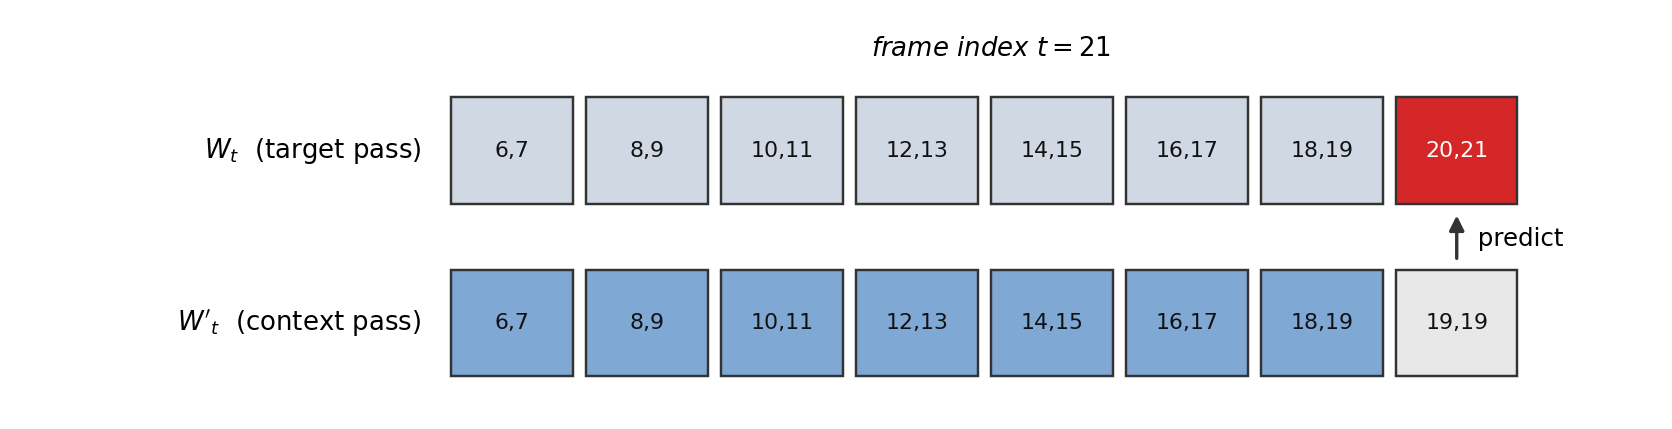
\includegraphics[width=\linewidth]{generated/fig_windows.png}
\caption{The two encoder passes used at frame $t$. Each box is one $2$-frame
tubelet, labelled by the frames it spans. The context pass $W'_t$ overwrites the
final tubelet with a repeat of $f_{t-2}$, so the predictor's context is a
function of $f_{\leq t-2}$ only, while the target comes from the full window
$W_t$. A single-pass implementation would let the context attend to
$f_{t-1},f_t$ and make the loss partly self-fulfilling.}
\label{fig:windows}
\end{figure}

\subsection{Baseline \texorpdfstring{$\mathcal{L}_1$}{L1}: information-matched
prediction error}

$\mathcal{L}_0$ and the geometry probes consume different representations ---
token grids versus a pooled vector --- which invites the objection that any
difference between them is an artefact of what they see. We therefore add a
second baseline that consumes \emph{exactly} the sequence the probes do. Let
$W^\star$ be a ridge map fitted to predict $z_t$ from its two predecessors,
\begin{equation}
W^\star = \arg\min_{W} \sum \bigl\lVert z_t - W[z_{t-1}; z_{t-2}] \bigr\rVert_2^2
+ \lambda \lVert W \rVert_F^2 , \qquad \lambda = 1,
\end{equation}
fitted on control-calibration clips only, and
$\mathcal{L}_1(t) = \lVert z_t - W^\star[z_{t-1};z_{t-2}] \rVert_2$. Scores for
the calibration clips themselves are produced by $5$-fold cross-fitting, so
$\mathcal{L}_1$'s own threshold is not optimistic. A probe must beat
\emph{both} baselines to count.

\subsection{Geometry probes}

All three are computed online from $\{z_t\}$ with no normalisation.

\begin{align}
\text{A. Trajectory curvature:}\quad
  a_t &= \bigl\lVert z_t - 2 z_{t-1} + z_{t-2} \bigr\rVert_2
  \label{eq:probeA}\\[2pt]
\text{B. Representational distance:}\quad
  b_t &= 1 - \frac{\langle z_t,\ \bar z_t \rangle}{\lVert z_t\rVert\,\lVert \bar z_t\rVert},
  \qquad \bar z_t = \tfrac{1}{5}\textstyle\sum_{i=1}^{5} z_{t-i}
  \label{eq:probeB}\\[2pt]
\text{C. Covariance shift:}\quad
  c_t &= \bigl\lVert \Sigma_t - \Sigma_{\mathrm{base}} \bigr\rVert_F,
  \qquad \Sigma_t = \widehat{\mathrm{Cov}}(z_{t-4..t})
  \label{eq:probeC}
\end{align}
where $\Sigma_{\mathrm{base}} = \widehat{\mathrm{Cov}}(z_{0..14})$ is frozen at
$t=14$, and both covariances use $\mathrm{ddof}=1$. Probe~A is a second
difference, probe~B is scale-invariant, probe~C compares second-order structure
against the clip's own pre-injection baseline.

\paragraph{Computing probe C without forming $d \times d$ matrices.}
Written naively, \eqref{eq:probeC} builds two $1024\times1024$ covariances per
frame. Both are low-rank: with centred factors $A \in \mathbb{R}^{k_a \times d}$
and $B \in \mathbb{R}^{k_b \times d}$ and $\Sigma = A^\top A/(k{-}1)$, the trace
identities give
\begin{equation}
\lVert \Sigma_a - \Sigma_b \rVert_F^2 =
\frac{\lVert AA^\top \rVert_F^2}{(k_a{-}1)^2}
- \frac{2\,\lVert AB^\top \rVert_F^2}{(k_a{-}1)(k_b{-}1)}
+ \frac{\lVert BB^\top \rVert_F^2}{(k_b{-}1)^2},
\end{equation}
which costs $O(k^2 d)$ instead of $O(d^2 k)$ and touches only $k \times k$
Grams. We verify it against the naive computation to machine precision
($\leq 2\times10^{-16}$ relative).

\paragraph{A numerical caveat.}
Probe~A is a second difference of nearby vectors, the textbook setting for
catastrophic cancellation: relative error in $z$ is amplified. Reduced-precision
inference is therefore not a free speed-up here, and we measure fp32 against
bf16 and fp16 on the actual probe values rather than assuming a choice is safe.

\section{Evaluation protocol}
\label{sec:protocol}

\subsection{Thresholds, and what ``fair'' means here}

Monitors live on incomparable scales --- a Frobenius norm and a cosine distance
have no common unit --- so comparing their raw scores is meaningless. What can
be matched is their false-alarm behaviour. For each monitor independently, the
threshold is the $99$th percentile of that monitor's scores pooled over the
\emph{control-calibration} clips and the evaluation frames. Every monitor
therefore raises false alarms on $1\%$ of control frames by construction, and
differences in detection latency are differences in sensitivity, not in scale.

Control clips are split into disjoint calibration ($n=\lgwNCalib$) and
evaluation ($n=\lgwNEval$) sets. Thresholds are set on the former and false
alarms measured on the latter; no threshold ever sees anomalous data.

\paragraph{A second operating point.}
Matching the \emph{per-frame} rate at $1\%$ compounds to roughly $14\%$ over a
$15$-frame episode, which no episode-level monitor could use. We therefore
repeat the entire analysis with thresholds re-derived so the \emph{clip-level}
false-alarm rate on calibration controls is $5\%$. This was fixed before any
inference run, and both regimes are reported unconditionally, so neither can be
selected after the fact.

\subsection{Detection latency as a survival quantity}

An alarm fires at the first evaluation frame whose score exceeds the threshold.
With injection at $t^\star = 15$ and an evaluation window of frames
$15..29$, detection latency is $\dt = t_{\text{alarm}} - 15 \in \{0,\dots,14\}$. A
clip that never alarms is \textbf{right-censored} at $14$: its latency is not
$14$, it is unobserved and at least $14$.

This censoring is the reason the protocol's headline metric needs a companion.
Once fewer than half the clips alarm, the median $\dt$ equals the censoring
value for \emph{every} monitor, and the pre-registered comparison returns ``no
difference'' no matter how large the true effect. We registered the median as
primary because it was specified in advance, and registered the
\textbf{restricted mean detection latency}
\begin{equation}
\RMTA \;=\; \mathbb{E}\bigl[\min(\dt, 14)\bigr] \;=\; \sum_{u=0}^{13} \widehat S(u),
\end{equation}
the area under the Kaplan--Meier curve $\widehat S$, as a secondary that stays
well defined at any detection rate. Lower is earlier.

\subsection{Tests}

\begin{itemize}
\item \textbf{Primary (as registered).} Paired Wilcoxon signed-rank on $\dt$,
probe versus baseline, one-sided (the hypothesis is directional), with censored
clips entered at $14$ --- conservative, since it understates differences. The
two-sided $p$ is always reported alongside, so the tail cannot be chosen post
hoc.
\item \textbf{Censoring-aware.} Log-rank on the Kaplan--Meier curves. Both arms
come from the same clips, violating its independence assumption, so it is
reported as corroborative only.
\item \textbf{Effect size.} Paired cluster bootstrap on the \RMTA{} difference
($\lgwNBoot$ resamples, the same resample applied to both monitors so that
pairing is preserved), giving a confidence interval in frames.
\item \textbf{Multiplicity.} Holm's step-down correction across all six
comparisons ($3$ probes $\times$ $2$ baselines), separately for the median and
\RMTA{} families.
\end{itemize}

\subsection{The decision gate}

A probe counts as a \textbf{faster detector} iff, against \emph{both} baselines, its
median $\dt$ is at least one frame lower \emph{and} the Holm-adjusted one-sided
$p$ is below $0.01$. If no probe qualifies, the protocol terminates the
expansion track and the result is written up as a negative one. The gate is
evaluated by code, not by reading tables.

\subsection{Pre-specified follow-up: what lives in the lag window}
\label{sec:mech}

If a probe does alarm before the loss, the frames in between are where the
representation has registered something the output error has not, and the
natural question is what. We pre-specify the analysis here so that it is fixed
before the lag window is known: fit linear probes to the latents $z_t$ for
$t \in [t^\star + \dt_{\text{probe}},\; t^\star + \dt_{\text{loss}})$, targeting
(i) which of the four anomalies was injected, and (ii) the disc's position and
velocity, which are the quantities the physics conditions actually change.

Two controls are part of the specification, because a linear probe on
high-dimensional latents is easy to over-read. Frames from one clip are highly
correlated, so a random train/test split lets the probe memorise clip identity
and return a near-perfect score that means nothing; all cross-validation is
therefore grouped by clip. And an accuracy is uninterpretable without a
reference, so every score is reported beside the majority-class rate and a
\emph{clip-level} label-shuffled control, which must land at chance. If the
shuffled control does not land at chance, the split is leaking and the real
score is not reported as evidence.

This analysis is contingent on the gate and is listed here as method, not
result.

\subsection{Guards against a vacuous verdict}

Two checks sit outside the hypothesis tests and exist to stop the gate from
being believed when it should not be.

\paragraph{Lift.} For every monitor we report
$\text{lift} = \text{detection rate} - \text{held-out clip false-alarm rate}$.
A monitor with lift near zero is firing at chance. If a \emph{baseline} fires at
chance, then beating it carries no information about H1 --- a probe cannot be shown to fire
\emph{sooner} than a signal that never fires --- and a passing
verdict is reported as \textsc{vacuous}. This check is not a hypothesis test and
does not alter any threshold or statistic; it only makes an existing failure
mode visible.

\paragraph{Causality, tested adversarially.} Claiming that frame $t$ cannot see
frame $t{+}1$ is cheap; testing it is not. For every registered adapter we take
a clip, invert every frame after a cut point, and assert that $z_t$,
$\mathcal{L}_0$ and all three probes are unchanged to floating-point tolerance
for $t$ at or before the cut. A separate test asserts that the $\mathcal{L}_0$
\emph{prediction} does not move when only $f_{t-1}$ and $f_t$ change, while
confirming it does move when $f_{t-2}$ changes --- so the guarantee is not
vacuously satisfied by a prediction that ignores its input. Probe streams are
additionally checked for prefix invariance: scores for frames $0..t$ must be
identical whether or not later frames exist.

\section{Benchmark}

\begin{figure}[t]
\centering
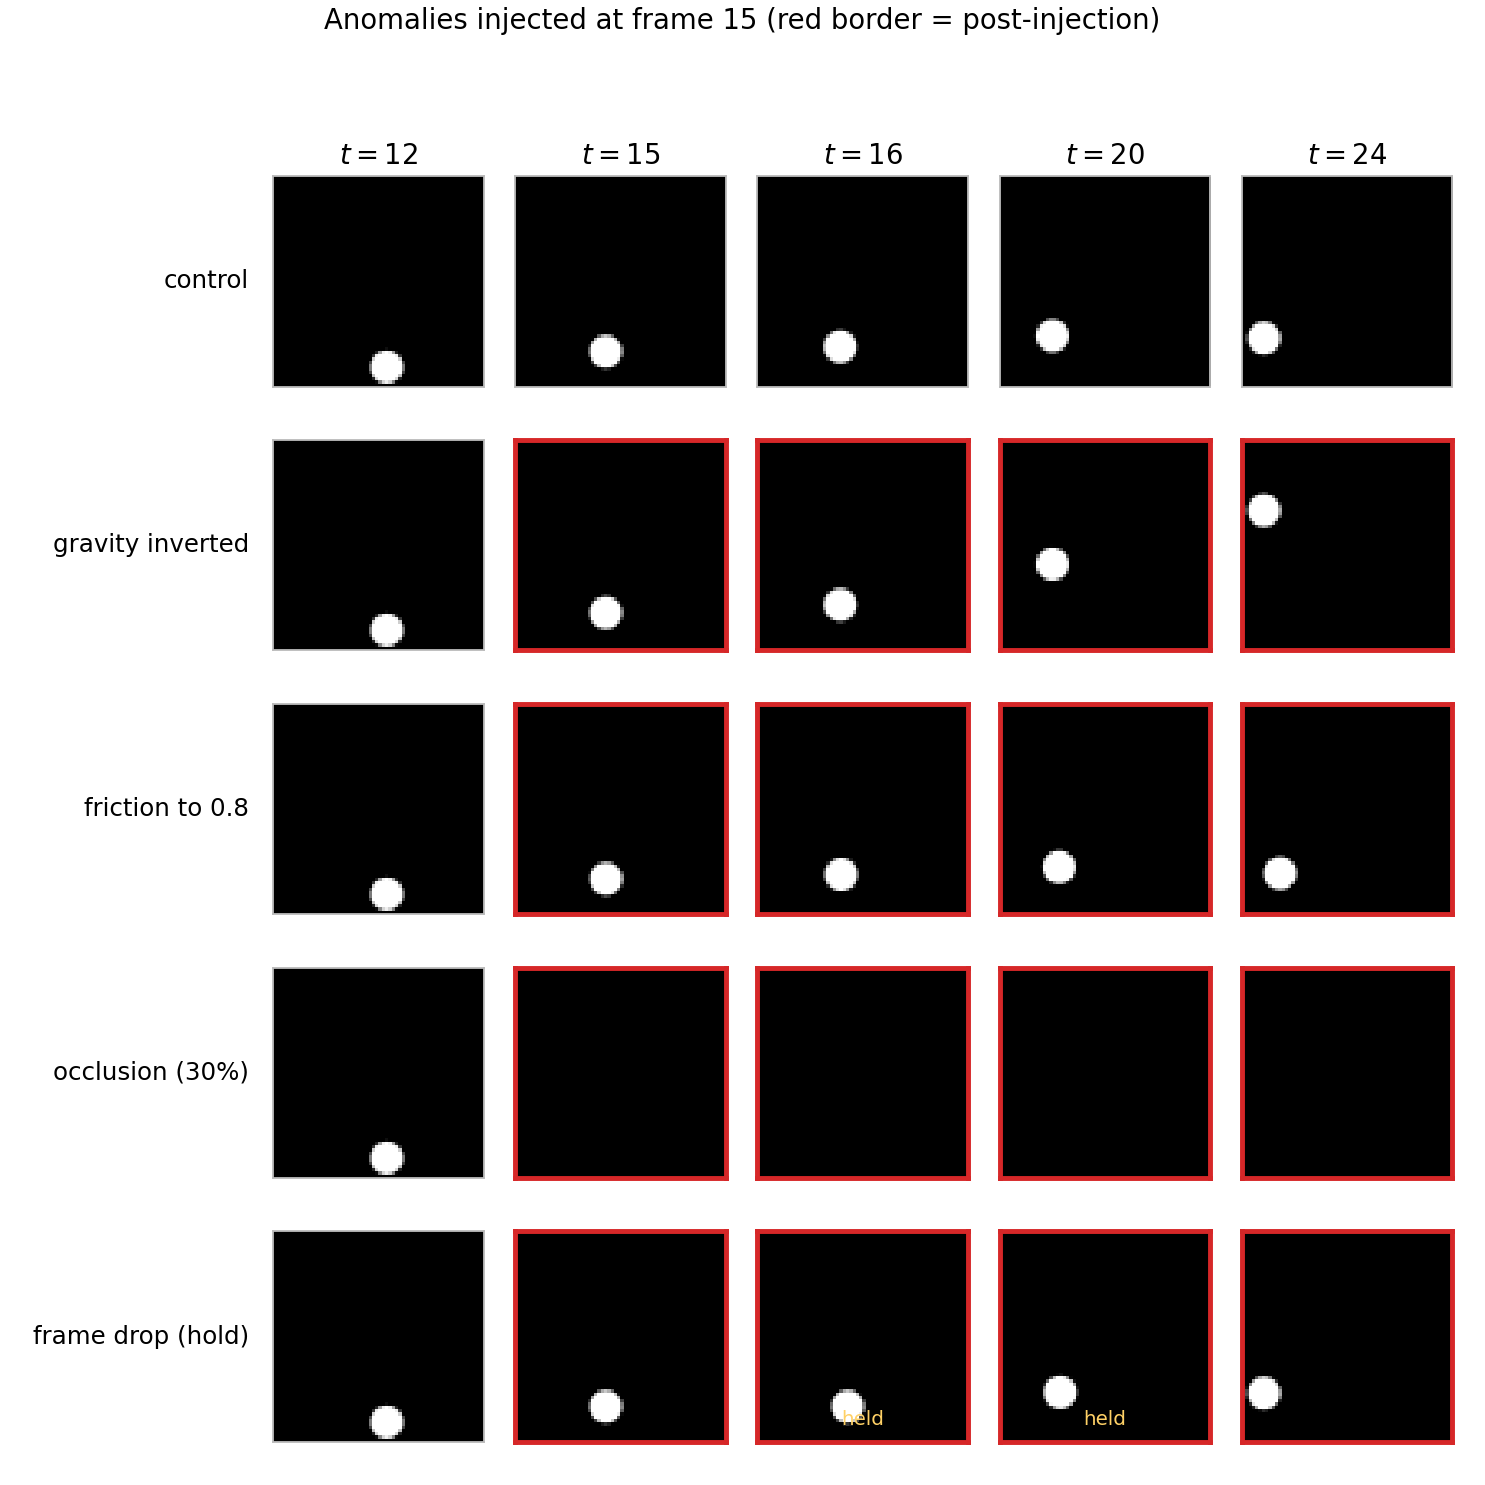
\includegraphics[width=0.86\linewidth]{generated/fig_dataset.png}
\caption{The four anomaly families, one row each, against the control row. Red
borders mark post-injection frames; ``held'' marks a frame the sensor glitch
repeats. All conditions share the control's pre-injection history exactly, so
every comparison is paired at the clip level.}
\label{fig:dataset}
\end{figure}

A disc of radius $5$ bounces inside a $64\times64$ frame for $30$ frames under
constant downward gravity $g_0 = 0.25\,\mathrm{px/frame^2}$ with perfectly
elastic collisions, so the baseline dynamics conserve energy and are
statistically stationary. Initial position, speed and direction are randomised;
generation is deterministic given the frozen seed.

At frame $t^\star=15$ one of four anomalies is injected
(Figure~\ref{fig:dataset}):

\begin{description}
\item[gravity inverted] $g \to -g_0$. Acceleration changes immediately;
position diverges only gradually, which makes this the subtlest condition at
short latency.
\item[friction] per-frame velocity retention $0.8^{1/5}$ and bounce restitution
$0.8$. Applied per frame rather than only at collisions, so the effect is
observable from the first post-injection frame; a collision-only version would
leave time-to-alarm undefined on clips with no bounce in the window.
\item[occlusion] a static black square of $29.9\%$ frame area, anchored on the
disc's path.
\item[frame drop] for underlying frames $15..22$, every other frame is not
delivered and the previous frame is held in its place --- four held frames ---
with normal delivery resuming at frame $23$.
\end{description}

\paragraph{What the occlusion condition actually tests.}
A $35\times35$ square anchored on the trajectory of a $10$-pixel disc does not
``partially block'' it. Measured across the condition,
\lgwOccFullyHidden{} of post-injection frames hide the disc completely,
\lgwOccPartial{} hide it partially, and in \lgwOccFullyHiddenClips{} of clips
the disc is never visible again inside the window. This condition therefore
probes object permanence --- does the representation register that a tracked
object has vanished --- rather than robustness to partial visual corruption. We
report it as such. It follows directly from the registered specification and is
not a defect, but describing it as partial occlusion would misstate what the
numbers mean.

\paragraph{Effect sizes are not comparable across conditions.}
Gravity inversion changes acceleration at once; friction changes velocity by
about $4.4\%$ per frame; occlusion removes the object; the frame drop freezes
it. These are different magnitudes of disturbance, so pooled results average
over heterogeneous effects, and per-condition results are reported separately.

\paragraph{Paired design.}
An anomalous clip and its control share a random seed, so their frames are
identical up to $t^\star$ and diverge only because of the injection. Every
monitor comparison is therefore within-clip, which is what the paired tests in
Section~\ref{sec:protocol} exploit.

\paragraph{Scale.}
The registered design is $1000$ anomalous clips ($250$ per condition) plus $200$
controls split into $\lgwNCalib$ calibration and $\lgwNEval$ evaluation. Clips
are bilinearly upsampled to the model's native resolution and replicated to
three channels.

\section{Results}
\label{sec:results}

\ifnum\lgwHasResults=0
\textit{No inference run has been analysed. Every table and number below is a
generated placeholder; see the note on the title page.}
\else
Run: \lgwModel, $n_{\text{anom}} = \lgwNAnom$, $d = \lgwDim$. Source:
\lgwSource. \lgwNote
\fi

At the pre-registered operating point, \texttt{loss\_L0} alarmed on 36.6\% of anomalous clips against a held-out clip-level false-alarm rate of 14.0\% (lift +0.226); \texttt{loss\_L1} alarmed on 70.8\% of anomalous clips against a held-out clip-level false-alarm rate of 10.0\% (lift +0.608).

Both baselines detect anomalies above chance, so the comparison against them is meaningful.

The strongest probe by RMTA is \texttt{probe\_B}, whose worst-case gain against either baseline is -2.05 frames; against \texttt{loss\_L0} its RMTA gain is +1.88 frames (95\% CI [+1.48, +2.26], Holm-adjusted $p=0.003$).

No probe satisfies the frozen Early Warner criterion (a median gain of at least one frame against both baselines at Holm-adjusted $p<0.01$).

Re-deriving thresholds so the clip-level false-alarm rate is 5\% rather than matching the per-frame rate does not change the picture: the Early Warner set becomes empty.


\begin{table}[t]
\centering
\small
\begin{tabular}{lrrrrrr}
\toprule
Monitor & median $\Delta t$ & RMTA & 95\% CI & detect. & clip FPR & lift \\
\midrule
$\mathcal{L}_0$ (V-JEPA 2 own loss) & 14.0 & 10.37 & [10.01, 10.70] & 0.366 & 0.140 & +0.226 \\
$\mathcal{L}_1$ (ridge, info-matched) & 4.0 & 6.45 & [6.08, 6.80] & 0.708 & 0.100 & +0.608 \\
\midrule
$\mathrm{A}$: curvature & 14.0 & 9.40 & [9.02, 9.75] & 0.424 & 0.120 & +0.304 \\
$\mathrm{B}$: repr.\ distance & 14.0 & 8.49 & [8.09, 8.89] & 0.490 & 0.130 & +0.360 \\
$\mathrm{C}$: covariance shift & 14.0 & 13.05 & [12.86, 13.23] & 0.179 & 0.040 & +0.139 \\
\bottomrule
\end{tabular}

\caption{Time-to-alarm per monitor at the pre-registered operating point
(per-frame false-alarm rate matched at $1\%$). \emph{Lift} is detection rate
minus held-out clip-level false-alarm rate; $\dagger$ marks a monitor firing at
chance. RMTA is the restricted mean time-to-alarm in frames, lower being
earlier, with a percentile bootstrap interval.}
\label{tab:tta}
\end{table}

\begin{table}[t]
\centering
\small
\begin{tabular}{lrrrrr}
\toprule
Comparison & median gain & RMTA gain & 95\% CI & $p$ (Holm) & $p$ (Holm, RMTA) \\
\midrule
\texttt{probe\_A\_vs\_loss\_L0} & +0.0 & +0.98 & [+0.70, +1.26] & $<10^{-4}$ & 0.003 \\
\texttt{probe\_A\_vs\_loss\_L1} & -10.0 & -2.95 & [-3.23, -2.68] & 1 & 1 \\
\texttt{probe\_B\_vs\_loss\_L0} & +0.0 & +1.88 & [+1.48, +2.26] & $<10^{-4}$ & 0.003 \\
\texttt{probe\_B\_vs\_loss\_L1} & -10.0 & -2.05 & [-2.33, -1.78] & 1 & 1 \\
\texttt{probe\_C\_vs\_loss\_L0} & +0.0 & -2.68 & [-3.05, -2.32] & 1 & 1 \\
\texttt{probe\_C\_vs\_loss\_L1} & -10.0 & -6.60 & [-7.00, -6.23] & 1 & 1 \\
\bottomrule
\end{tabular}

\caption{Paired probe-versus-baseline comparisons. Positive gain means the
probe alarms earlier. $p$ values are Holm-adjusted across all six comparisons;
the RMTA column uses the paired cluster bootstrap. A probe is an Early Warner
only if it achieves a median gain of at least one frame against \emph{both}
baselines at adjusted $p<0.01$.}
\label{tab:cmp}
\end{table}

\begin{figure}[t]
\centering
\IfFileExists{generated/fig_survival.png}{%
  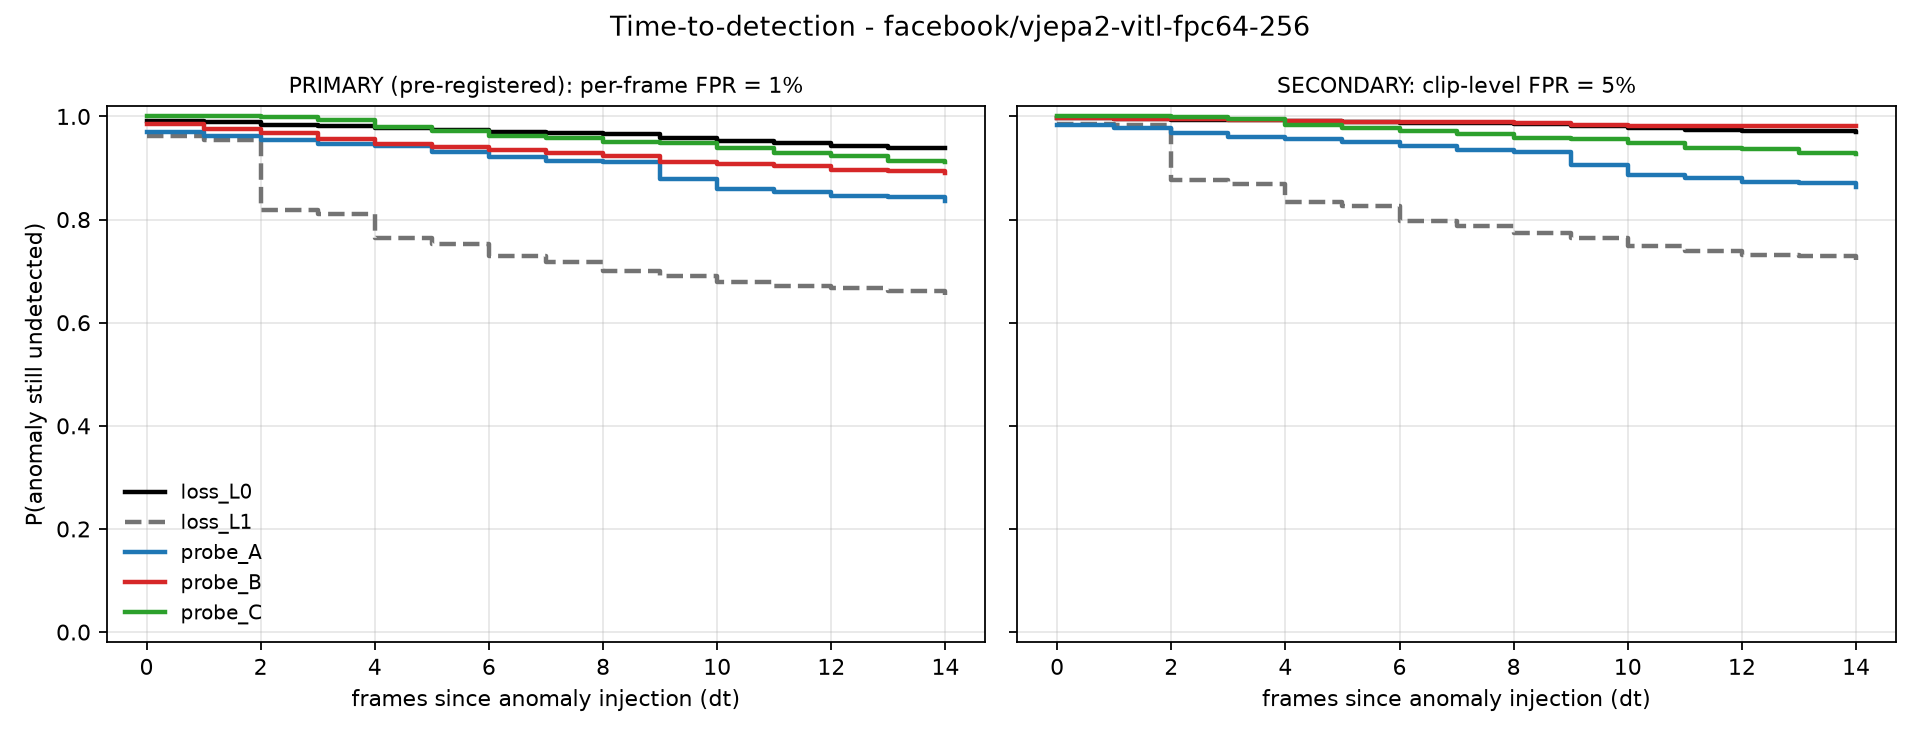
\includegraphics[width=\linewidth]{generated/fig_survival.png}}{%
  \fbox{\parbox{0.8\linewidth}{\centering\vspace{18pt}\textsc{pending}\\[2pt]
  \footnotesize survival curves are produced by the analysis run\vspace{18pt}}}}
\caption{Kaplan--Meier curves for time-to-detection under both threshold
regimes: the probability that an anomaly remains undetected $\dt$ frames after
injection. A monitor that warns earlier drops sooner. Curves that stay flat
near $1$ indicate a monitor that mostly fails to fire inside the window, which
is the regime in which the median is uninformative.}
\label{fig:survival}
\end{figure}

\begin{table}[t]
\centering
\small
\begin{tabular}{lrrrr}
\toprule
Monitor & gravity inv. & friction & occlusion & frame drop \\
\midrule
$\mathcal{L}_0$ (V-JEPA 2 own loss) & 12.59 & 13.08 & 13.59 & 2.23 \\
$\mathcal{L}_1$ (ridge, info-matched) & 10.56 & 12.74 & 1.50 & 0.98 \\
\midrule
$\mathrm{A}$: curvature & 13.62 & 13.56 & 8.95 & 1.45 \\
$\mathrm{B}$: repr.\ distance & 13.14 & 12.86 & 4.88 & 3.10 \\
$\mathrm{C}$: covariance shift & 13.43 & 13.62 & 12.72 & 12.42 \\
\bottomrule
\end{tabular}

\caption{RMTA by anomaly condition (frames; lower is earlier). Conditions
differ in disturbance magnitude, so these are not comparable across columns ---
they show \emph{where} any effect is concentrated, not which anomaly is
``easier''.}
\label{tab:cond}
\end{table}

\begin{table}[t]
\centering
\small
\begin{tabular}{lrrrr}
\toprule
Monitor & median $\Delta t$ & RMTA & detect. & clip FPR \\
\midrule
$\mathcal{L}_0$ (V-JEPA 2 own loss) & 14.0 & 10.67 & 0.330 & 0.100 \\
$\mathcal{L}_1$ (ridge, info-matched) & 7.0 & 7.21 & 0.621 & 0.020 \\
\midrule
$\mathrm{A}$: curvature & 14.0 & 10.09 & 0.357 & 0.080 \\
$\mathrm{B}$: repr.\ distance & 14.0 & 9.44 & 0.408 & 0.040 \\
$\mathrm{C}$: covariance shift & 14.0 & 12.94 & 0.194 & 0.050 \\
\bottomrule
\end{tabular}

\caption{The secondary operating point: thresholds re-derived so the
clip-level false-alarm rate on calibration controls is $5\%$. Registered before
any inference run and reported unconditionally.}
\label{tab:secondary}
\end{table}

\subsection{Reading these tables honestly}

Three questions should be asked of Table~\ref{tab:tta} before
Table~\ref{tab:cmp} is read at all.

\emph{Do the baselines detect anything?} If a baseline's lift is near zero it
fires at chance, and every comparison against it in Table~\ref{tab:cmp} is
uninformative about the hypothesis regardless of its $p$ value. The
$\dagger$ marker and the \textsc{vacuous} flag exist for this case.

\emph{Is the median degenerate?} If detection rates are below $50\%$, the median
$\dt$ column will read identically for every monitor and the median-gain column
of Table~\ref{tab:cmp} will be all zeros. That is an artefact of censoring, not
evidence of equality; the RMTA columns are the ones carrying information.

\emph{Does the conclusion survive the second operating point?} A result that
appears at a $1\%$ per-frame threshold and vanishes at a $5\%$ clip-level
threshold is an operating-point artefact, not a property of the
representation.

\subsection{Gate}

The frozen decision rule returns \textbf{\lgwVerdict}. Early warners under the
registered primary: \lgwEarlyWarners. Under the censoring-robust secondary:
\lgwRmtaWarners. Median degenerate: \lgwMedianDegenerate. Baselines firing at
chance: \lgwBaselinesAtChance. Verdict vacuous: \lgwVacuous.

\section{The harness as the reusable artefact}

The question in this paper is one instance of a template: \emph{does some
internal signal of a frozen sequence model move before its output error does?}
Answering it for another architecture, another anomaly family or another probe
should not require rebuilding the protocol, and if it does, the resulting
numbers will not be comparable to ours.

\paragraph{What is shared and what is pluggable.}
The causal loop --- which frames frame $t$ may see, where the context window
stops, which frames receive a prediction loss --- is identical for every
architecture and is implemented exactly once. A model supplies two methods:

\begin{quote}
\code{encode\_window(windows) -> (latent, loss\_target)} \\
\code{predict\_final\_step(context\_windows) -> prediction}
\end{quote}

\noindent
The windows handed to both are already the causal and context windows of
Section~\ref{sec:method}, so a new adapter cannot accidentally read the future:
the information boundary is enforced by the caller, not by the contributor's
discipline. Probes, thresholds, survival statistics, multiplicity correction and
the gate are then shared verbatim. Adding V-JEPA 2 takes roughly twenty-five
lines beyond preprocessing; a model with no native prediction head returns
\code{None} and is scored against $\mathcal{L}_1$ alone.

\paragraph{Contributions are held to the contract automatically.}
Every registered adapter is run through a parameterised test suite: output
shapes, the loss window, prefix invariance, the future-inversion causality
check, and the assertion that the prediction is blind to the frames it predicts
while still responding to $f_{t-2}$. Registering an adapter without supplying a
cheap constructor for these tests fails the suite by design, so an architecture
cannot silently enter the benchmark without being held to the same standard as
the others. This is what licenses a cross-architecture comparison: the
difference between two rows is a difference between models, not between
pipelines.

\paragraph{Reproducibility.}
The dataset is generated deterministically from a frozen seed, so no data needs
to be distributed and no version can drift. The frozen constants are pinned by a
test that fails if any of them is edited. Each run records its own metadata, and
the analysis emits the full result set --- both threshold regimes, both metric
families, per-condition breakdowns, false-alarm rates and the gate verdict ---
in a single JSON from which every table and numeric sentence in this paper is
regenerated. No number here is transcribed by hand, which removes an entire
class of silent error between the experiment and the manuscript.

\paragraph{Scope of the claim.}
We make no claim that these three probes are the best possible geometric
monitors, nor that this synthetic domain is representative of deployment. The
reusable part is the protocol that decides such questions without accidentally
answering them in advance.

\section{Limitations}
\label{sec:limitations}

\paragraph{No registered result yet.}
The first and largest limitation is that the central question is unanswered.
This version contributes a protocol, a benchmark and a set of documented failure
modes; it does not contribute a measurement of detection latency in V-JEPA 2.
Until the registered run executes, every claim here is about the apparatus.

\paragraph{Sudden onset measures latency, not anticipation.}
Anomalies are injected abruptly at a known frame, so a monitor can only react to
something that has already happened. This design cannot distinguish a monitor
that detects quickly from one that anticipates, and we make no anticipation
claim. Work on \emph{anticipated} latents \citep{samad2026puls} addresses the
other regime, where the quantity of interest is a model's forward prediction
rather than its reaction. A gradual-onset benchmark would be needed to speak to
anticipation, and we do not have one.

\paragraph{Synthetic clips.}
A single disc on a black background at $64 \times 64$ is a deliberately
controlled setting: it makes the injection frame exact, the pre-injection
histories matched, and the ground truth available. It is also nothing like
deployment. Scene complexity, texture, camera motion, multiple objects and
natural statistics are all absent, and any result here is a statement about this
regime only.

\paragraph{One model family.}
The registered experiment covers frozen V-JEPA 2. A VideoMAE adapter exists and
passes the contract suite, but \emph{has not been run} --- an adapter is a
capability, not a result, and we are careful not to present one as the other.
Whether any effect is a property of joint-embedding predictive architectures, of
video transformers generally, or of one checkpoint is not decided here.

\paragraph{The occlusion family measures object permanence.}
Our occlusion condition hides the disc completely in \lgwOccFullyHidden{} of
post-injection frames, so it asks whether the representation registers that a
tracked object has vanished. \citet{xie2026tracking} show that this regime
dissociates sharply inside V-JEPA 2: the predictor forgets moving hidden objects
within about $0.3$~seconds while the encoder retains such information for far
longer. Since our geometry probes read pooled encoder states and
$\mathcal{L}_0$ reads the predictor, that dissociation is a plausible confound
for this family specifically, and results on it should be interpreted against
their finding rather than as a clean test of the hypothesis.

\paragraph{Mean pooling discards where the anomaly is.}
Both the latent state and the $\mathcal{L}_0$ loss average over the spatial
token grid. Our anomalies are spatially local, so averaging dilutes them. On two
clips of real pretrained weights, $\mathcal{L}_0$ spanned only about $\pm 2\%$,
which is the observation behind the lift diagnostic: if that holds at scale,
$\mathcal{L}_0$ may alarm at chance and comparisons against it would be vacuous.
Max-pooling, or a loss restricted to tokens whose content actually changed, are
natural variants we did not register.

\paragraph{Probes A and C may carry per-clip offsets.}
In the same two-clip check, probe~C differed by roughly $8\%$ between clips
while moving only a few percent \emph{within} each. With thresholds pooled
across clips, a monitor whose between-clip variance exceeds its within-clip
signal behaves partly as a per-clip constant rather than a change detector.
Probe~B, scale-invariant by construction, showed no comparable offset.
Standardising each probe against its own pre-injection frames is the standard
remedy, but it cannot be applied uniformly here because probe~C is undefined
before frame~15 and so has no within-clip reference window. We flag this rather
than patch it: changing a frozen probe definition after seeing data is exactly
what pre-registration exists to prevent.

\paragraph{Pooled thresholds assume stationarity in $t$.}
For $t<15$ the causal window is left-padded by repeating $f_0$, so warm-up
latents are computed on partly synthetic windows and the score distribution is
mildly $t$-dependent. Controls and anomalies pass through an identical pipeline,
so this cannot manufacture a difference \emph{between} monitors, but it widens
the pooled calibration distribution and costs sensitivity. A per-frame threshold
would be the cleaner estimator.

\paragraph{Latency is quantised by the tubelet.}
Since $z_t$ summarises frames $(t-1,t)$, latencies should not be read as
single-frame reaction times. Both monitor families inherit the same
quantisation, so comparisons stay fair, but absolute numbers are coarser than
the units suggest.

\paragraph{The log-rank test is mis-specified here.}
Both arms come from the same clips, violating its independence assumption. It is
reported as corroborative only; the paired Wilcoxon and the paired cluster
bootstrap respect the design.

\paragraph{A null result would be about these probes.}
If no probe clears the gate, the honest conclusion is that \emph{these three
second-order summaries of a mean-pooled latent} are not faster than prediction
error on \emph{this} benchmark --- not that no geometric signal exists. The
space of candidate probes is large; we fixed three in advance precisely so we
could not search it.

\section{Future work}
\label{sec:future}

\paragraph{Run the registered experiment.}
The immediate next step is the one this paper is missing: execute the frozen
protocol at $256$~px and report the verdict, whichever way it falls. The
estimated cost is about one GPU-hour. Everything needed is written and tested.

\paragraph{Compression and detection latency (drafted, deliberately not run).}
The natural follow-up becomes available only once a monitoring harness exists.
\citet{fu2026quantization} report that post-training quantization of a world
model produces \emph{asymmetric} sensitivity across components, and failure
modes that further optimization does not repair. A mean-performance number hides
that; a per-anomaly-family detection-latency measurement should not.

We have drafted a second study asking whether compression changes \emph{which}
anomalies a model still catches and \emph{how fast}, rather than degrading it
uniformly. Its shape:

\begin{itemize}
\item Six precisions (fp32, bf16, fp16, int8 weight-only, W8A8, 4-bit
weight-only) crossed with three placements (encoder only, predictor only,
both). Placement is the factor that tests the asymmetry claim directly: under
encoder-only compression the latents the probes consume are degraded while the
prediction head is intact, and vice versa.
\item One primary contrast per anomaly family, Holm-corrected across the four,
with every other cell exploratory and labelled as such.
\item \textbf{Equivalence testing}, not null-hypothesis testing. The interesting
claim is usually that compression does \emph{not} hurt, which is an equivalence
claim and cannot be supported by failing to reject a difference. The draft
specifies TOST on the latency difference --- and leaves the equivalence margins
blank, as an explicit TODO for the author to set and justify before freezing,
because choosing a margin after seeing the effect is the easiest way to
manufacture an equivalence result.
\item A fresh seed for the confirmatory clips, so that no clip used to develop
the harness appears in the confirmatory set, and per-cell threshold calibration,
so that a shift in score scale is not confounded with a change in sensitivity.
\item A second-GPU arm. Quantization kernels, tensor-core paths and accumulation
order differ across hardware, so a compression effect that does not reproduce on
two GPUs is a kernel artefact rather than a property of the model.
\item Two exploratory analyses: \emph{blind spots} --- whether misses
concentrate in one anomaly family rather than thinning uniformly --- and
\emph{motion energy}, testing whether compression costs concentrate in
low-motion clips where there is least signal to work with. Both target the same
idea, that aggregate accuracy can hold while the distribution of failures
shifts.
\end{itemize}

The draft is marked \textsc{draft, not frozen} and no data may be collected
under it until its margins are set and it is frozen in its own commit. It does
not amend the v1 pre-registration, which remains in force untouched. We record
it here so that its existence and date are on the record and it cannot later be
presented as having been registered earlier than it was.

\paragraph{Other directions.}
A physics-simulator domain with contact and articulation would test whether
anything here survives outside synthetic discs. A gradual-onset benchmark would
let the anticipation question be asked properly, rather than the latency
question we can currently answer. And the per-clip standardisation issue raised
in Section~\ref{sec:limitations} deserves a clean treatment: a probe family
defined to be invariant to per-clip offsets from the start, rather than one
patched after the fact.

\section{Conclusion}

We set out to measure whether the internal geometry of a frozen video world
model crosses an alarm threshold sooner than the model's own prediction error,
and built the experiment so the answer could come out either way. That
measurement is \pending: it needs about one GPU-hour of credit, not any missing
code. We report the apparatus, and what building it revealed.

The methodological point stands independently of the eventual verdict. A
comparison between an internal signal and an output error is unusually easy to
settle in advance without noticing: by letting the baseline's context attend to
the frames it predicts; by calibrating thresholds on the data they are scored
against; by summarising a censored latency with a statistic that is constant
under censoring; or by beating a baseline that never fires. We made the first
structurally impossible and tested it adversarially, the second impossible by
construction, the third visible through a registered secondary, and the fourth
visible through a lift check that marks an otherwise-passing verdict vacuous.

Two further findings came from building rather than from measuring. Our
occlusion condition, specified as a square covering $30\%$ of the frame, in
practice hides the disc entirely in \lgwOccFullyHidden{} of post-injection
frames --- so it probes object permanence, a regime in which the encoder and
predictor of V-JEPA 2 are known to dissociate \citep{xie2026tracking}, and
describing it as partial occlusion would have misstated what the numbers mean.
And implementing a second architecture showed that the leakage trap is
architecture-specific: VideoMAE builds its targets by patchifying whatever
tensor it is handed, reaching the same bias by an entirely different route.
Whether a loss is causal has to be re-asked, and re-tested, per architecture; it
is not a property a harness can confer.

None of these guards is sophisticated. What they share is that omitting any one
of them yields a cleaner-looking result, which is why we think they belong in
the protocol rather than in the discussion. To our knowledge the lift check in
particular is not standard in representation-based anomaly detection, though the
collapse it guards against is documented \citep{pavuluri2026asleep}.

We release the harness as a benchmark that another architecture joins in about
twenty-five lines and is then held to the same contract automatically, so that
the next claim of this shape can be checked rather than argued --- including
ours, once the run happens.

\section*{Reproducibility statement}

The protocol was frozen before any code was written and is reproduced in
Appendix~\ref{app:prereg}; every subsequent change is logged with its date and
the evidence that motivated it. The dataset is generated deterministically from
a single seed, so none is distributed. Frozen constants are pinned by a test
that fails if edited. The causality and leakage guarantees are tested, not
asserted. Every table, figure and numeric sentence in this paper is generated
from a run's result JSON by a script in the repository; with no run analysed,
the manuscript compiles with visible \textsc{pending} markers rather than
plausible values, which is why no registered number appears above.


\bibliography{refs}

\appendix
\section{Frozen protocol and change log}
\label{app:prereg}

\subsection{What was frozen, and when}

The protocol was frozen on 2026-10-06 before any code was written. It fixes:
the dataset (resolution, length, injection frame, the four anomaly definitions,
the control split), the five monitors and their closed forms, the threshold
rule, the time-to-alarm metric, the statistical tests, the multiplicity
correction, and the decision gate with its termination branch. The full text
ships with the repository.

\subsection{Contradictions in the source specification, resolved before freezing}

Three requirements could not all hold simultaneously. Each was resolved before
any code ran and the resolution was itself frozen.

\begin{description}
\item[Constant velocity versus inverted gravity.] A constant-velocity baseline
has no gravity to invert. Resolved by giving the baseline a constant downward
$g_0$ with perfectly elastic collisions, which keeps the dynamics stationary and
makes $g \to -g_0$ well defined.

\item[Friction with no observable effect.] A restitution change applied only at
collisions may not manifest before the evaluation window closes, leaving
time-to-alarm undefined on a substantial fraction of clips. Resolved by applying
a per-frame drag in addition to the restitution change.

\item[A per-frame latent under a two-frame tubelet.] V-JEPA 2 has no
representation that is a function of a single frame. Resolved by the sliding
causal window of Section~\ref{sec:method}, which is a function of $f_{\leq t}$
and whose final tubelet spans $(t{-}1,t)$.
\end{description}

\subsection{Changes after freezing}

\paragraph{Before any inference run.}
\begin{enumerate}
\item The Wilcoxon tail was fixed as one-sided primary, with the two-sided value
always reported. The hypothesis is directional, and the tail had to be fixed
before seeing data.
\item Two secondary analyses were registered: the restricted mean time-to-alarm
with a paired cluster bootstrap, and a clip-matched $5\%$ false-alarm-rate
threshold regime. Both weaknesses follow from the \emph{definition} of the
primary metric rather than from any observed result --- a censored median is
degenerate below $50\%$ detection, and $1\%$ per frame compounds to roughly
$14\%$ per clip over fifteen frames. The primary metric and the gate were not
changed.
\item $\mathcal{L}_1$'s scores on calibration clips were specified to come from
$5$-fold cross-fitting, so that its own threshold is not optimistic.
\end{enumerate}

\paragraph{After a two-clip correctness check on real weights.}
The lift column, the at-chance flag and the \textsc{vacuous} marker were added.
What had been observed at that point was score \emph{magnitude} --- that
$\mathcal{L}_0$ spanned about $\pm2\%$ --- and not any time-to-alarm, gate
outcome or effect direction. No threshold, metric, test or gate criterion was
altered; the addition only makes an existing failure mode visible in the report.
We record the provenance here rather than omitting it, so that a reader can
judge the timing for themselves.

\subsection{Falsification}

The hypothesis is falsified if every geometry probe has a median $\dt$ greater
than or equal to that of $\mathcal{L}_0$, or if no difference reaches
Holm-adjusted $p<0.01$. The protocol commits in that case to terminating the
expansion track and reporting the negative result.


\end{document}
